\documentclass[11pt]{article}
\usepackage{graphicx}
\usepackage{float}
\usepackage{cite}
\usepackage{url}
\usepackage{caption}

\title{Mastering Essential Unix Tools and LaTeX Utilities}
\author{Fouad Hammad}
\date{\today}

\begin{document}
	
	\maketitle
	
	\begin{abstract}
		In the world of Unix-based systems, mastering fundamental tools can be essiential to mastering and understanding the Unix interface. This paper will explore five powerful utilities—LaTeX/BibTeX for document preparation, \texttt{tar} for file archival, \texttt{less} and \texttt{more} for file viewing, \texttt{import} for image capturing, and \texttt{awk} for text processing. Each of these tools play a vital role in the Unix toolkit and can be useful across programming, scripting, and documentation usages.
	\end{abstract}
	
	\section{Introduction}
	Unix systems provide a feature-rich set of tools that can be combined to perform complex tasks effectively. This paper will reflect on five essential tools learned in this course that have significantly improved my own workflow in programming and technical writing.
	
	\section{LaTeX and BibTeX}
	LaTeX is a powerful markup language for document preparation. It allows precise control over document layouts, mathematical equations, tables, figures, and more. BibTeX is used alongside LaTeX to manage references.
	
	\subsection*{Example Table in LaTeX}
	\begin{table}[H]
		\centering
		\begin{tabular}{|c|c|}
			\hline
			Tool & Purpose \\
			\hline
			LaTeX & Document preparation \\
			BibTeX & Reference management \\
			tar & Archiving \\
			awk & Pattern scanning \\
			\hline
		\end{tabular}
		\caption{Sample Tools and Their Uses}
	\end{table}
	
	\subsection*{Reference Example}
	This table and document is an example of what can be done in LaTeX \cite{latex}.
	
	\section{The \texttt{tar} Command}
	The \texttt{tar} command is used to archive multiple files and directories into a single file. This can be combined with \texttt{gzip} to allow for efficient compression of large datasets and/or projects:
	\begin{verbatim}
		tar -cvf archive.tar file1 file2
		tar -xvf archive.tar
	\end{verbatim}
	This makes it ideal for packaging projects such as this paper submission.
	
	\section{Using \texttt{less} and \texttt{more}}
	When viewing large text files, commands like \texttt{less} and \texttt{more} allow navigation without opening an editor. For instance:
	\begin{verbatim}
		less largefile.txt
		more errorlog.txt
	\end{verbatim}
	These tools are especially helpful when browsing documentation or logs.
	
	\section{Capturing Screens with \texttt{import}}
	The \texttt{import} command allows for screen capturing directly from the terminal. The following command saves a screenshot:
	\begin{verbatim}
		import screenshot.png
	\end{verbatim}
	\begin{figure}[H]
		\centering
		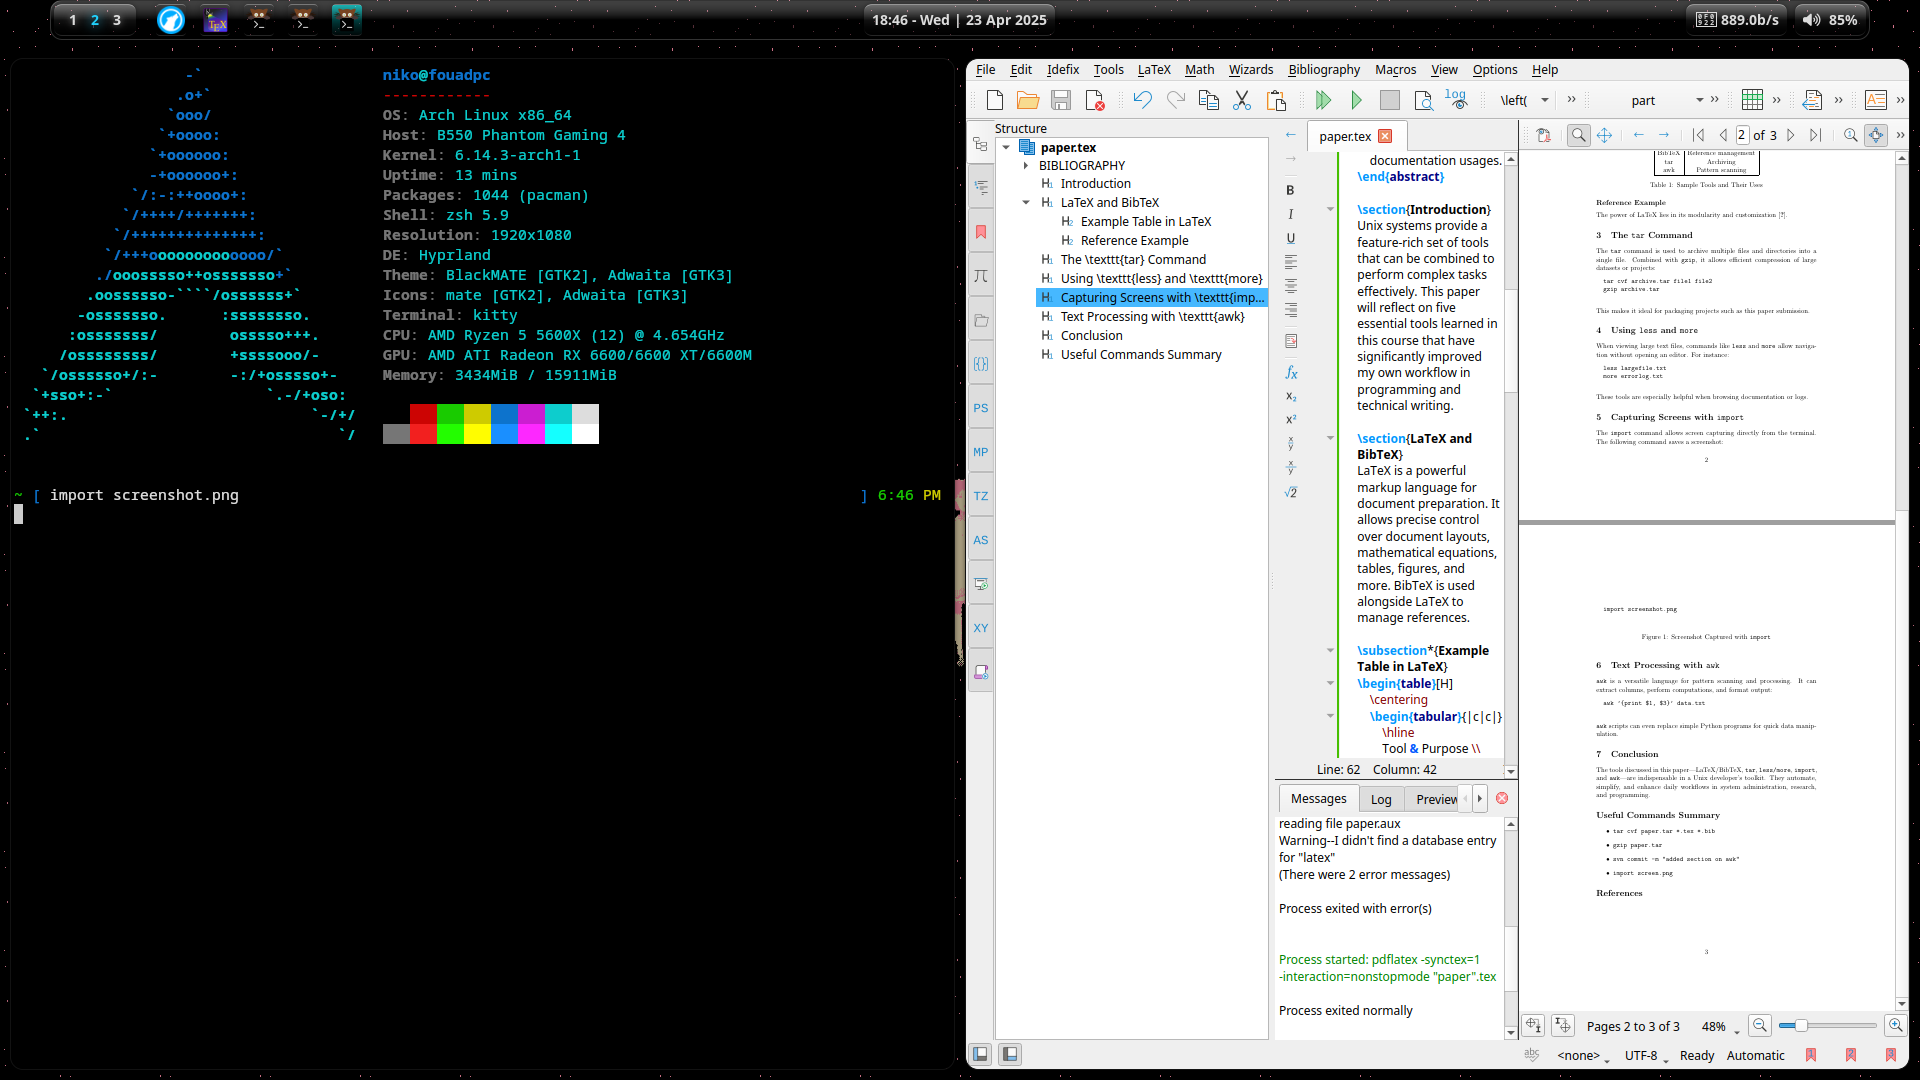
\includegraphics[width=0.6\textwidth]{screenshot.png}
		\caption{Screenshot Captured with \texttt{import}}
	\end{figure}
	
	\section{Text Processing with \texttt{awk}}
	\texttt{awk} is a versatile command or rather language for pattern scanning and processing. It can extract columns, perform computations, and format output:
	\begin{verbatim}
		awk '{print $1, $3}' data.txt
	\end{verbatim}
	\texttt{awk} scripts can even replace simple Python programs for quick data manipulation\cite{awk}.
	
	\section{Conclusion}
	The tools discussed in this paper—LaTeX/BibTeX, \texttt{tar}, \texttt{less/more}, \texttt{import}, and \texttt{awk}—are indispensable in a Unix developer’s toolkit. In fact, they are so useful on their own that they are even used here in this document. Here,they automate, simplify, and enhance daily workflows in system administration, research, and programming in order to effciently and effectively get the job done. 
	
	\section*{Useful Commands Summary}
	\begin{itemize}
		\item \texttt{tar cvf paper.tar *.tex *.bib}
		\item \texttt{gzip paper.tar}
		\item \texttt{import screen.png}
	\end{itemize}
	
	\bibliographystyle{plain}
	\bibliography{refs}
	
\end{document}
